%%%%%%%%%%%%%%%%%%%%%%%%%%%%%%%%%%%%%%%%%%%%%%%%%%%%%%%%
%%%%%%%%%%%%%%%%%%%%%%%%%%%%%%%%%%%%%%%%%%%%%%%%%%%%%%%%
%%%                                                  %%%
%%% University of Arizona themed Beamer presentation %%%
%%% Based on the Warsaw, Palo Alto and UNL templates %%%
%%% modified by Joseph V. Casillas (6-13-2011)       %%%
%%%                                                  %%%
%%%%%%%%%%%%%%%%%%%%%%%%%%%%%%%%%%%%%%%%%%%%%%%%%%%%%%%%
%%%%%%%%%%%%%%%%%%%%%%%%%%%%%%%%%%%%%%%%%%%%%%%%%%%%%%%%

\documentclass{beamer}
\mode<presentation>{\usetheme{UA3}\setbeamercovered{transparent}}
\usepackage[english,spanish]{babel}
\usepackage[utf8]{inputenc}
\usepackage{tipa}
\usepackage{t1enc}
\usepackage{amssymb}   
\usepackage{soul}		
\usepackage{graphicx}	
\usepackage{colortbl}
\usepackage{url}		
\usepackage{qtree}	
\usepackage{cgloss4e}	
\usepackage{verbatim}
\usepackage{media9}
\usepackage{tikz-qtree}
\usepackage[notocbib]{apacite}
\usepackage{textcomp}
\usepackage{multirow}
\usepackage{apacite}
\usepackage{natbib}	
\usepackage{hyperref}
\usepackage{times}


\title{Percepción del habla}

\author[Casillas]{Joseph Casillas}

\institute{Universidad de Arizona}

\date{Semana 10}

\subject{Linguistics}

\begin{document}

%%%%%%%%%%%%%%%%%%%%%%%%%%%%%%%%%
%%%%%%%%%%%%%%%%%%%%%%%%%%%%%%%%%
\begin{frame}%Página principal
  \titlepage
\end{frame}

\begin{frame}
	\frametitle{La percepción del habla}
	\framesubtitle{Repaso}

	\begin{enumerate}
	\itemsep=.7em
		\item ¿Qué es VOT? ¿Cómo difiere /b/ de /p/? ¿Y /t/ (español) de /t/ (inglés)? 
		\item ¿Qué significa ``la ausencia de invarianza''? ¿Por qué supone un problema a la hora de explicar la percepción del habla?
		\item En vuestras propias palabras, ¿qué es la percepción categórica?
		\item ¿Cuál es el procedimiento para un experimento 2AFC (2-alternative forced choice)?
		\item ¿Cuál es el procedimiento para un experimento de discriminación?
		\item ¿Cuál es el procedimiento para un experimento de acceso léxico?
		\item ¿Qué es una tarea online? ¿Cómo difiere de una tarea offline? Da ejemplos. 
	\end{enumerate}
\end{frame}


\begin{frame}
	\frametitle{La percepción del habla}
	\framesubtitle{Pallier et al. (1997)}
	
	\begin{itemize}
		\item ¿Quiénes son los participantes? 
		\item ¿Por qué los escogieron? 
		\item ¿Qué lenguas hablan? 
		\item ¿Cuál es la parte crucial para este experimento?
		\item ¿Qué metodología utiliza \cite{Pallier1997a}?
	\end{itemize}
\end{frame}

\begin{frame}
	\frametitle{La percepción del habla}
	\framesubtitle{Pallier et al. (1997)}
	
	\begin{itemize}
		\item Bilingües secuenciales tempranos: español/catalán, catalán español
		\item El catalán cuenta con un contraste vocálico que no existe en español (\textipa{/e/-/\textepsilon/})
	\end{itemize}
\end{frame}

\begin{frame}
	\frametitle{La percepción del habla}
	\framesubtitle{Pallier et al. (1997)}
	
	\begin{center}
		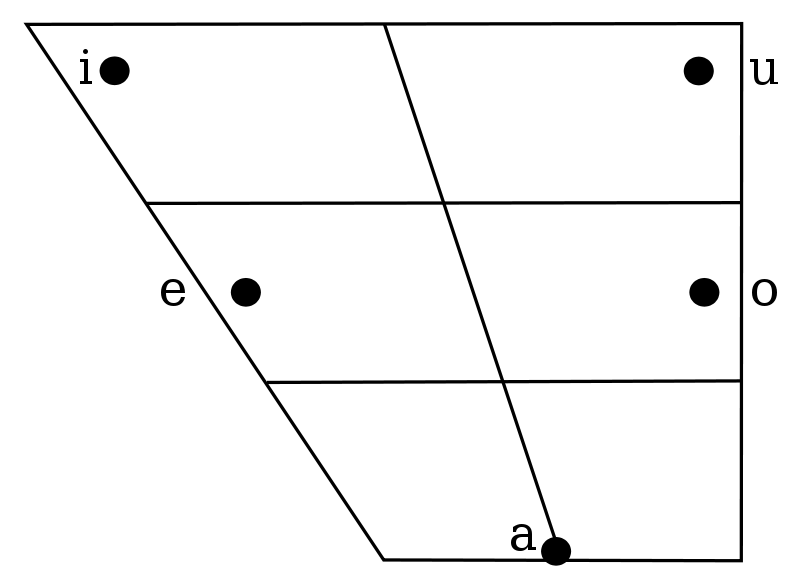
\includegraphics[scale=.2]{figures/spanish.png} 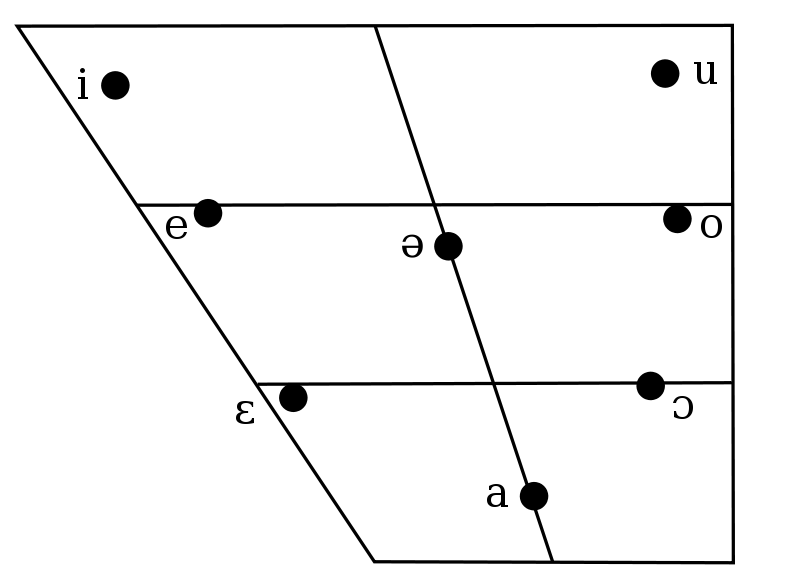
\includegraphics[scale=.2]{figures/catalan.png}
	\end{center}
\end{frame}

\begin{frame}
	\frametitle{La percepción del habla}
	\framesubtitle{Pallier et al. (1997)}
	
	\begin{itemize}
		\item Bilingües secuenciales tempranos: español/catalán, catalán español
		\item El catalán cuenta con un contraste vocálico que no existe en español (\textipa{/e/-/\textepsilon/})
		\item Identificación (2AFC) \\
		``¿Escuchaste \textipa{[\textprimstress pe.\textfishhookr a]} (Peter) o \textipa{[\textprimstress pE.\textfishhookr a]} (pera)?''
		\item Discriminación \\
		``¿Son iguales o son diferentes?''
	\end{itemize}
\end{frame}

\begin{frame} 
	\frametitle{La percepción del habla}
	\framesubtitle{Pallier et al. (1997)}
	
	\begin{center}
		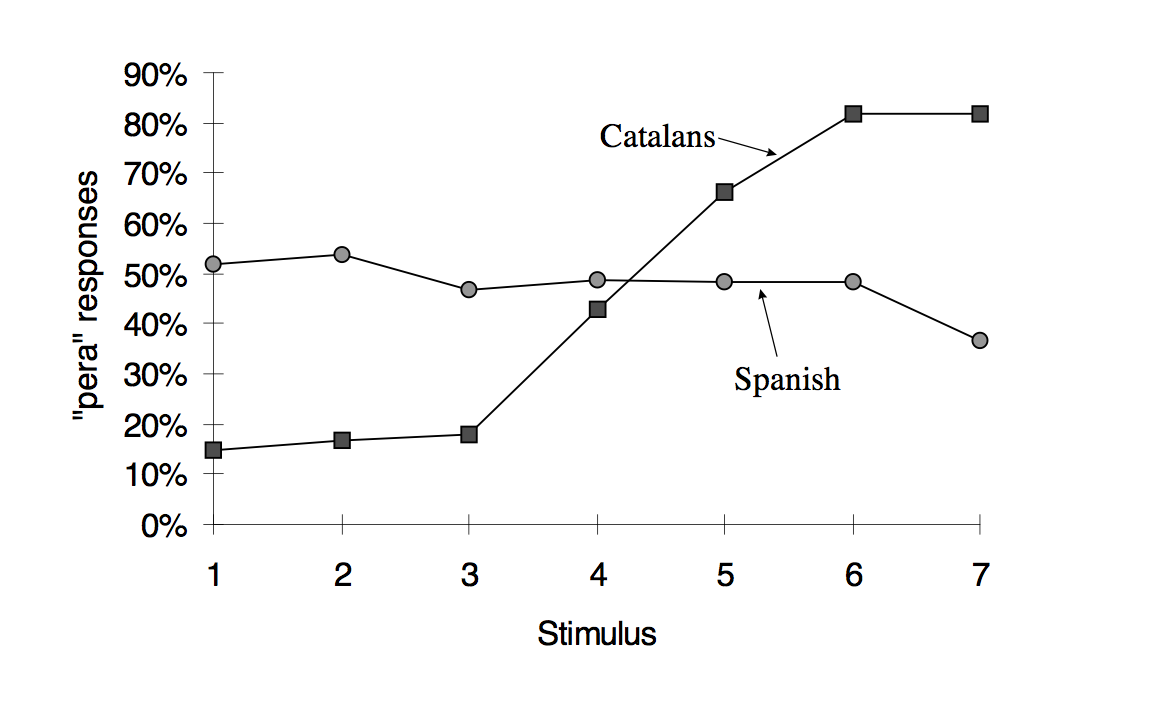
\includegraphics[scale=.25]{figures/pallier1.png}
	\end{center}
\end{frame}

\begin{frame} 
	\frametitle{La percepción del habla}
	\framesubtitle{Pallier et al. (1997)}
	
	\begin{center}
		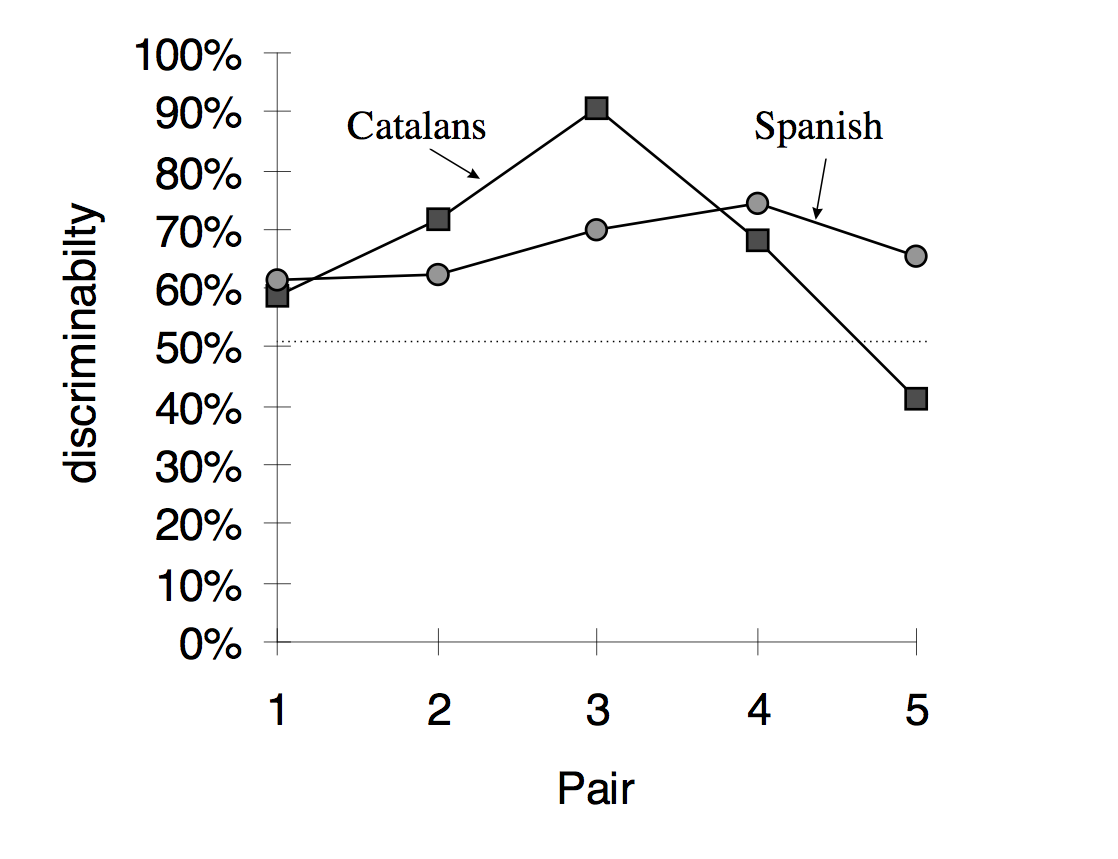
\includegraphics[scale=.25]{figures/pallier2.png}
	\end{center}
\end{frame}

\begin{frame} 
	\frametitle{La percepción del habla}
	\framesubtitle{Pallier et al. (1997)}
	
	Conclusión
	\begin{itemize}
		\item 
	\end{itemize}
\end{frame}
	
\begin{frame} 
	\frametitle{La percepción del habla}
	\framesubtitle{Pallier et al. (1997)}
	
	Conclusión
	\begin{itemize}
		\item Los bilingües tempranos español/catalán no dominan el contraste entre los fonemas \textipa{/e/-/E/}
		\item Estar expuesto a una edad temprana (durante el periodo sensible) no parece ser suficiente
	\end{itemize}
\end{frame}




\begin{frame}
	\frametitle{La percepción del habla}
	\framesubtitle{Barrios et al. (2010)}
	
	\begin{itemize}
		\item ¿Quiénes son los participantes? 
		\item ¿Por qué los escogieron? 
		\item ¿Qué lenguas hablan? 
		\item ¿Cuál es la parte crucial para este experimento?
		\item ¿Qué metodología utiliza \cite{Barrios2010}?
	\end{itemize}
\end{frame}

\begin{frame}
	\frametitle{La percepción del habla}
	\framesubtitle{Barrios et al. (2010)}
	
	\begin{center}
		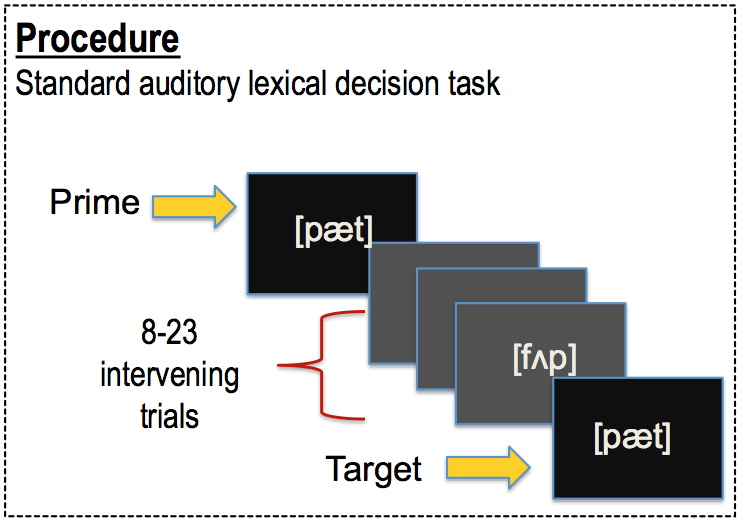
\includegraphics[scale=.25]{figures/barrios1.png}
	\end{center}
\end{frame}

\begin{frame}
	\frametitle{La percepción del habla}
	\framesubtitle{Barrios et al. (2010)}
	
	\begin{center}
		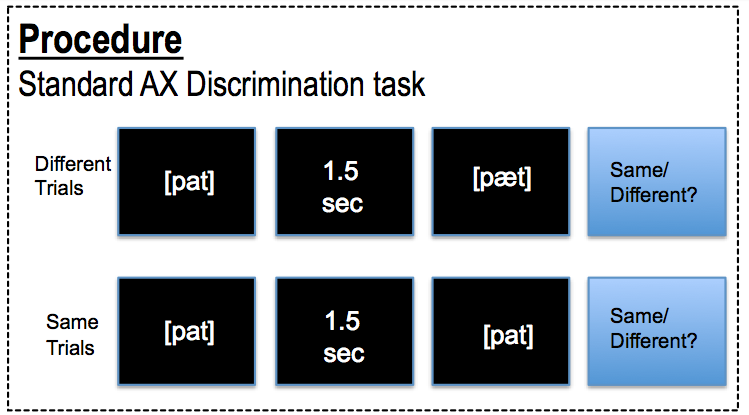
\includegraphics[scale=.25]{figures/barrios2.png}
	\end{center}
\end{frame}

\begin{frame}
	\frametitle{La percepción del habla}
	\framesubtitle{Barrios et al. (2010)}
	
	\begin{center}
		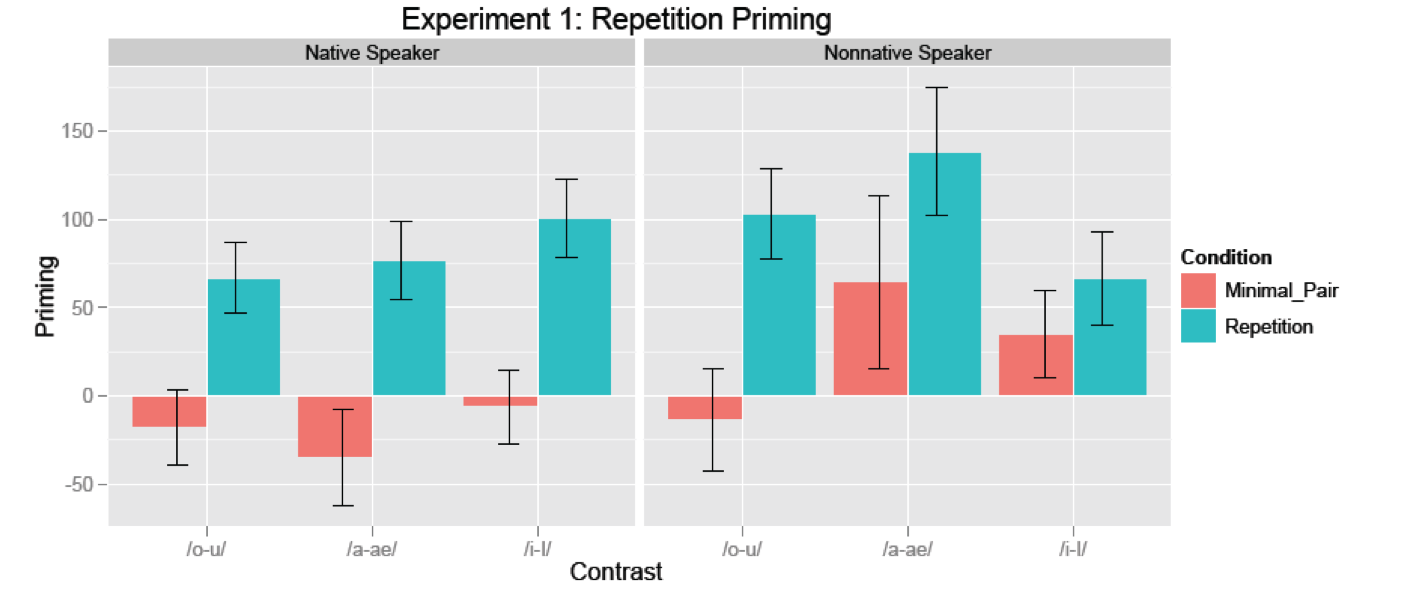
\includegraphics[scale=.25]{figures/barrios3.png}
	\end{center}
\end{frame}

\begin{frame}
	\frametitle{La percepción del habla}
	\framesubtitle{Barrios et al. (2010)}
	
	\begin{center}
		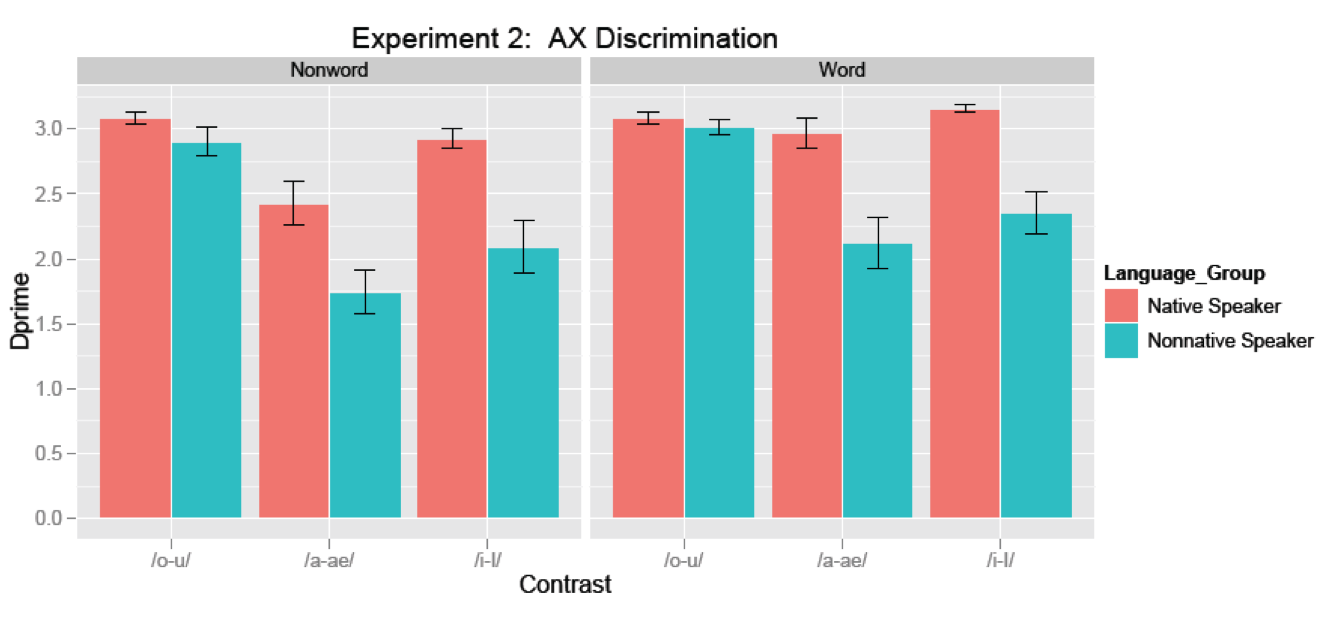
\includegraphics[scale=.25]{figures/barrios4.png}
	\end{center}
\end{frame}

\begin{frame}
	\frametitle{La percepción del habla}
	\framesubtitle{Barrios et al. (2010)}
	
	\begin{itemize}
		\item Estos bilingües tardíos (que tienen mucha experiencia en su L2) tratan algunos pares mínimos del inglés como homófonos. 
	\end{itemize}
\end{frame}



\begin{frame}
	\frametitle{La percepción del habla}
	\framesubtitle{Sebastián-Gallés et al. (2006)}
	
	\begin{itemize}
		\item ¿Quiénes son los participantes? 
		\item ¿Por qué los escogieron? 
		\item ¿Qué lenguas hablan? 
		\item ¿Cuál es la parte crucial para este experimento?
		\item ¿Qué metodología utiliza \cite{Sebastian-Galls2006}?
	\end{itemize}
\end{frame}


\begin{frame} 
	\frametitle{La percepción del habla}
	\framesubtitle{Sebastián-Gallés et al. (2006)}
	
	Experimento de acceso léxico
		\begin{itemize}
		\item Explota el contraste \textipa{/\textipa{e}/} -- \textipa{/\textepsilon/} utilizando palabras falsas basadas en palabras reales \\
		\begin{center}
		\begin{tabular}{lll}
		\textcolor{UAred}{/\textipa{g\textschwa \textturny\textepsilon d\textschwa}/} & $\rightarrow$ & \textcolor{UAred}{*/\textipa{g\textschwa \textturny ed\textschwa}/} \\
		\textcolor{UAred}{/\textipa{u\textturny er\textschwa s}/} & $\rightarrow$ & \textcolor{UAred}{*/\textipa{u\textturny\textepsilon r\textschwa s}/} \\
		\end{tabular}
		\end{center}
	\end{itemize}
\end{frame}

\begin{frame} 
	\frametitle{La percepción del habla}
	\framesubtitle{Sebastián-Gallés et al. (2006)}
	
	\begin{center}
		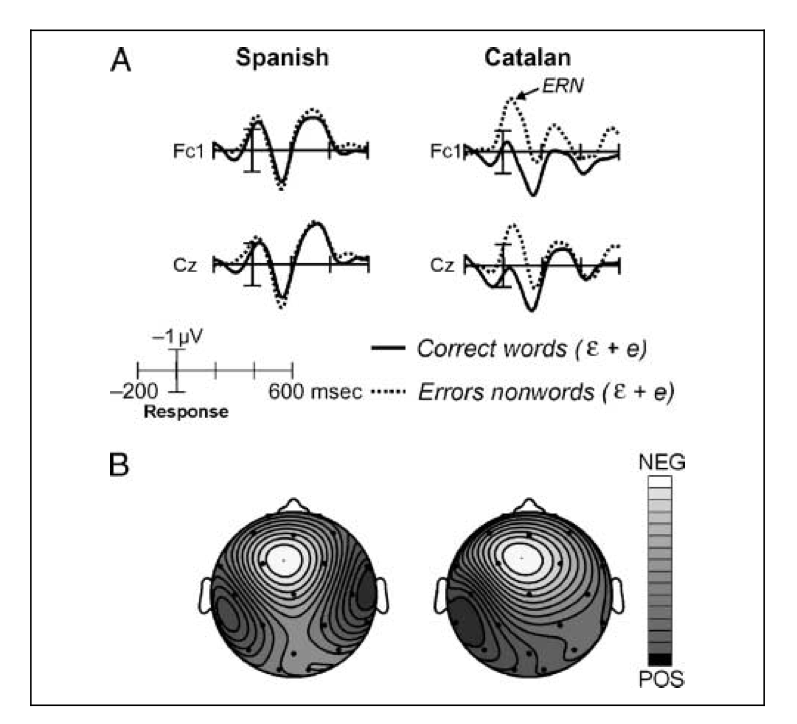
\includegraphics[scale=.25]{figures/sebas.png}
	\end{center}
\end{frame}

\begin{frame} 
	\frametitle{La percepción del habla}
	\framesubtitle{Sebastián-Gallés et al. (2006)}
	
	\begin{itemize}
		\item Los bilingües hispanodominantes no perciben bien el contraste 
		\item No presentan la misma activación neuronal (ERP) para las palabras falsas 
		\item Conclusión: incluso para los bilingües tempranos, una de las dos lenguas siempre es dominante con respecto a la otra
	\end{itemize}
\end{frame}

\begin{frame}[allowframebreaks]{References}
	\bibliographystyle{apacite}
	\bibliography{lib}
\end{frame}
\end{document}